%!TEX program = xelatex
\documentclass[11pt,a4paper]{article}
\usepackage[utf8]{inputenc}
\usepackage[T1]{fontenc}
\usepackage{authblk}
\usepackage{ctex}
\usepackage{tikz}
\usepackage{pgfplots}
\usepackage{verbatim}
\usepackage{amsfonts}
\usepackage{amsmath}
\usepackage{amsthm}
\usepackage{indentfirst}
\usepackage{amssymb}
\setlength{\parindent}{0pt}
\usetikzlibrary{shapes,snakes}
\newcommand{\argmax}{\operatornamewithlimits{argmax}}
\newcommand{\argmin}{\operatornamewithlimits{argmin}}
\DeclareMathOperator{\col}{col}
\usepackage{booktabs}
\newtheorem{theorem}{Theorem}
\newtheorem{note}{Note}
\newtheorem{definition}{Definition}
\newtheorem{proposition}{Proposition}
\newtheorem{lemma}{Lemma}
\newtheorem{example}{Example}
\newtheorem{corollary}{Corollary}
\usepackage{graphicx}
\usepackage{geometry}
\usepackage{hyperref}
\newcommand{\code}{	exttt}
\geometry{a4paper,scale=0.8}
\title{STAT 425 Note 1}
\author[*]{Wenxiao Yang}
\affil[*]{Department of Mathematics, University of Illinois at Urbana-Champaign}
\date{2021}

\usepackage{listings}
\usepackage{xcolor}

\lstset{numbers=left,numberstyle=\tiny,keywordstyle=\color{blue},commentstyle=\color[cmyk]{1,0,1,0},frame=single,escapeinside=``,extendedchars=false,xleftmargin=2em,xrightmargin=2em,aboveskip=1em,tabsize=4,showspaces=false}






\begin{document}
\maketitle
\tableofcontents
\newpage


\section{Review of statistics}
\subsection{Random Vectors}
\subsubsection{Mean}
$$\mu =\mathbb{E}(\mathbf{Z})=\begin{pmatrix}
    \mathbb{E}(Z_1)\\
    \mathbb{E}(Z_2)\\
    \cdots\\
    \mathbb{E}(Z_m)
\end{pmatrix}$$
\subsubsection{Variance-Covariance matrix}
$$\Sigma_{m\times m}=Cov(\mathbf{Z})=\mathbb{E}((\mathbf{Z}-\mu)(\mathbf{Z}-\mu)^T)=\begin{bmatrix}
    Var(Z_1)&\cdots	&Cov(Z_1,Z_m)\\
    \cdots&\cdots	&\cdots\\
    Cov(Z_m,Z_1)&\cdots &Var(Z_m)
\end{bmatrix}$$
\subsection{Affine Transformation}
(1)
$$\mathbf{W}=\mathbf{a}_{n\times 1}+\mathbf{B}_{n\times m}\mathbf{Z}_{m\times 1}$$
$$\mathbb{E}(\mathbf{W})=\mathbf{a}+\mathbf{B}\mu,\ Cov(\mathbf{W})=\mathbf{B}\Sigma \mathbf{B}^T$$
(2)
$$\mathbf{W}=\mathbf{v}^T \mathbf{Z}=v_1Z_1+...+v_mZ_m$$
$$\mathbb{E}(\mathbf{W})=\mathbf{v}^T\mu=\sum_{i=1}^mv_i\mu_i$$ $$Var(\mathbf{W})=\mathbf{v}^T\Sigma \mathbf{v}=\sum_{i=1}^mv_i^2Var(Z_i)+2\sum_{i<j}v_iv_jCov(Z_i,Z_j)$$
$$\text{i.e. }\mathbb{E}(\mathbf{A}\mathbf{Z})=\mathbf{A}\mathbb{E}(Z);\ Var(\mathbf{A}\mathbf{Z})=\mathbf{A}Var(\mathbf{Z})\mathbf{A}^T$$
(3)
$$Cov(\mathbf{A}\mathbf{X},\mathbf{B}\mathbf{Y})=\mathbb{E}[(\mathbf{A}\mathbf{X}-\mathbf{A}\mathbb{E}(X))(\mathbf{B}\mathbf{Y}-\mathbf{B}\mathbb{E}(Y))^T]=\mathbf{A}\mathbb{E}[(\mathbf{X}-\mathbb{E}(X))(\mathbf{Y}-\mathbb{E}(Y))^T]\mathbf{B}^T=\mathbf{A}Cov(\mathbf{X},\mathbf{Y})\mathbf{B}^T$$































\section{Regression Analysis (SLR)}
It is a "tool" used to examine the relationship between
a \textbf{Dependent Variable} or \textbf{Response} $Y$, and
one (or more) \textbf{Independent Variables} or \textbf{Regressors} or \textbf{Predictors} $X_1 ,X_2 ,...,X_p$.

\subsection{Simple Linear Regression}
$$y=\beta_0+\beta_1 x$$
$\beta_0$ is the *intercept*; $\beta_1$ is the *slope*.
One Response $\mathcal{Y}$; One Predictor $\mathcal{X}$
The data come in pairs:
$$\begin{aligned}
&x_1\quad &y_1\\&x_2\quad &y_2\\&\vdots\quad &\vdots\\&x_n\quad &y_n
\end{aligned}$$
$Y$ is a RANDOM VARIABLE that has a distribution for every level of the independent variable.

\subsection{Simple Linear Regression Model}
$$y_i=\beta_0+\beta_1 x_i+\varepsilon_i $$
where the *intercept* $\beta_0$, the *slope* $\beta_1$, and the *error variance* $\sigma^2$ are the *model parameters*.

\subsubsection{Assumptions of errors $\varepsilon$: 1. Mean zero, 2. umcorrelated, 3. homoscedastic}
The \textit{errors} $\varepsilon_1 , \varepsilon_2 , . . . , \varepsilon_n$ are assumed to\\
– have \textit{mean zero}: $E(\varepsilon_i ) = 0$\\
– be \textit{uncorrelated}: $Cov(\varepsilon_ i , \varepsilon_ j ) = 0, i \neq j$\\
– be \textit{homoscedastic}: $Var(\varepsilon_i ) = \sigma^ 2$ does not depend on $i$.\\

The last two could be combined and written as:
$$Cov(\varepsilon_1,\varepsilon_j)=\sigma^2\delta_{ij}$$
where $\delta_{ij}=\left\{\begin{matrix}
    0&i\neq j\\
    1&i=j
\end{matrix}\right.$

\subsubsection{Assumptions on $Y|X$}
Based on the SLR model moment assumptions on the error terms, we have the following assumptions for the moments of $Y $conditioning on $X$:\\
1. $E(y_i|x_i)=\beta_0+\beta_1x_i$\\
2. $Var(y_i|x_i)=\sigma^2$\\
3. $Cov(y_i,y_j|x_i,x_j)=0,\ i\neq j$
\subsubsection{Interpretation of $\beta_1$, $\beta_0$}
$\beta_1$ is the \textbf{change in the mean} of the probability distribution function of $y$ per unit change in $x$.\\
When $x=0$, $\beta_0$ is the \textbf{mean} of the probability distribution function of $y$(at $x=0$), otherwise $\beta_0$ \textbf{has no particular meaning}.\\

\subsection{Least Squares}
We want to find estimates of $\beta_0$, $\beta_1$ to minimize:
$$\min [y_i-E(y_i)]\Leftrightarrow \min [y_i-(\beta_0+\beta_1 x_i)]$$
minimize the \textbf{Residual Sum of Squares (RSS)}
$$RSS=\sum_{i=1}^n(y_i-\beta_0-\beta_1 x_i)^2$$
$$(\hat{\beta_0},\hat{\beta_1})=\argmin_{(\beta_0,\beta_1)}RSS$$

$$\begin{aligned}
    \frac{\partial RSS}{\partial \beta_0}=0 &\Leftrightarrow -2\sum_{i=1}^n(y_i-\beta_0-\beta_1 x_i)=0\\
    & \Leftrightarrow \beta_0 n+\beta_1\sum_{i=1}^n x_i=\sum_{i=1}^n y_i
\end{aligned}$$
$$\begin{aligned}
    \frac{\partial RSS}{\partial \beta_1}=0 &\Leftrightarrow -2\sum_{i=1}^n(y_i-\beta_0-\beta_1 x_i)x_i=0\\
    &\Leftrightarrow \beta_0 \sum_{i=1}^nx_i+\beta_1\sum_{i=1}^n x_i^2=\sum_{i=1}^n x_iy_i
\end{aligned}$$

\subsubsection{LS Estimators}
Then we can solve that
$$\begin{aligned}
&\hat{\beta}_{1}=\frac{\sum_{i=1}^{n} x_{i} y_{i}-n \bar{x} \bar{y}}{\sum_{i=1}^{n} x_{i}^{2}-n \bar{x}^{2}}=\frac{\sum_{i=1}^{n}\left(x_{i}-\bar{x}\right)\left(y_{i}-\bar{y}\right)}{\sum_{i=1}^{n}\left(x_{i}-\bar{x}\right)^{2}}=\frac{\sum_{i=1}^{n}\left(x_{i}-\bar{x}\right)y_{i}}{\sum_{i=1}^{n}\left(x_{i}-\bar{x}\right)^{2}} \\
&\hat{\beta}_{0}=\bar{y}-\hat{\beta}_{1} \bar{x}
\end{aligned}$$

Alternative Representation of $\hat{\beta_1}$
$$\hat{\beta}_{1}=\frac{\sum_{i}\left(x_{i}-\bar{x}\right)\left(y_{i}-\bar{y}\right)}{\sum_{i}\left(x_{i}-\bar{x}\right)^{2}}=\frac{S_{x y}}{S_{x x}}=r_{x y} \sqrt{\frac{S_{y y}}{S_{x x}}}$$
Where 
\begin{equation}
    \begin{aligned}
        &S_{xy}=\sum_{i}\left(x_{i}-\bar{x}\right)\left(y_{i}-\bar{y}\right); &S_{xx}=\sum_{i}\left(x_{i}-\bar{x}\right)^{2}\\
        &S_{yy}=\sum_{i}\left(y_{i}-\bar{y}\right)^{2}; &r_{xy}=\frac{\sum_{i}\left(x_{i}-\bar{x}\right)\left(y_{i}-\bar{y}\right)}{\sqrt{\sum_{i}\left(x_{i}-\bar{x}\right)^{2}\sum_{i}\left(y_{i}-\bar{y}\right)^{2}}}=\frac{S_{xy}}{\sqrt{S_{xx}S_{yy}}}
    \end{aligned}
    \nonumber
\end{equation}

\subsubsection{Fitted Values \& Residuals}
The \underline{\textit{Prediction of $y_i$}} or the \underline{\textit{fitted value at $x_i$}}
$$\hat{y_i}=\hat{\beta_0}+\hat{\beta_1}x_i$$
$$\hat{y_i}=\bar{y}+\hat{\beta_1}(x_i-\bar{x})=\bar{y}+\frac{\sum_{i=1}^{n}\left(x_{i}-\bar{x}\right)\left(y_{i}-\bar{y}\right)}{\sum_{i=1}^{n}\left(x_{i}-\bar{x}\right)^{2}}(x_i-\bar{x})$$
The \underline{\textit{$i^{th}$ residual}}
$$r_i=y_i-\hat{y_i}$$

\subsubsection{Properties of residuals}
1. $\sum_i r_i=0$\\
2. $RSS=\sum_i r_i^2$ is minimized\\
3. $\sum_{i=1}y_i=\sum_{i=1}\hat{y_i}$\\
4. $\sum_ix_ir_i=0$ 一阶导条件(proof: $\sum_ix_ir_i=\sum_ix_i(y_i-\bar{y}-\hat{\beta_1}(x_i-\bar{x}))=\sum_ix_iy_i-n\bar{x}\bar{y}-\frac{\sum_{i=1}^{n} x_{i} y_{i}-n \bar{x} \bar{y}}{\sum_{i=1}^{n} x_{i}^{2}-n \bar{x}^{2}}(\sum_ix_i^2-n\bar{x}^2)=0$)\\
5. $\sum_i \hat{y_i} r_i=0$ (inferred from 4)\\
6. The regression line always goes through the point $(\bar{x},\bar{y})$.

\subsubsection{Degree of freedom}
The \textbf{degree of freedom(df)} of the residuals is
$$df=\textit{(Sample size)}-\textit{(\# of parameters)}$$
$df=2$ in this case.

\subsubsection{(Sample) Error variance}
The error variance is estimated by$$\hat{\sigma}^2=\frac{1}{n-2}\sum_i r_i^2$$

\subsection{Goodness of Fit: $R-$square}
\subsubsection{TSS, RSS, FSS}
$TSS: \sum_i(y_i-\bar{y})^2$\\
$RSS: \sum_ir_i^2$\\
$FSS: \sum_i(\hat{y}_i-\bar{y})^2$
$$\begin{aligned}
    \sum_{i}\left(y_{i}-\bar{y}\right)^{2} &=\sum_{i}\left(y_{i}-\hat{y}_{i}+\hat{y}_{i}-\bar{y}\right)^{2}=\sum_{i}\left(r_{i}+\hat{y}_{i}-\bar{y}\right)^{2} \\
    &=\sum_{i} r_{i}^{2}+\sum_{i}\left(\hat{y}_{i}-\bar{y}\right)^{2} \\
    T S S &=R S S+F S S
    \end{aligned}$$
\subsubsection{Cofficient of Determination($R^2$)}
$$R^{2}=\frac{\sum_{i}\left(\hat{y}_{i}-\bar{y}\right)^{2}}{\sum_{i}\left(y_{i}-\bar{y}\right)^{2}}=\frac{F S S}{T S S}=\frac{T S S-R S S}{T S S}=1-\frac{R S S}{T S S}$$
$0\leq R^2\leq 1$\\
It measures the effect of $X$ in reducing the variation in $Y$.\\
The larger $R^2$ is, the more the total variation of $y$ is reduced by reducing the independent variable $x$.\\

$R^2$ can also represent the degree of linear association between $X$ and $Y$.\\
$r_{xy}= \pm \sqrt{R^2}$, where the sign is the sign of the slope.
\begin{equation}
    \begin{aligned}
       r_{xy}^2
       &=\frac{(\sum_{i}\left(x_{i}-\bar{x}\right)\left(y_{i}-\bar{y}\right))^2}{\sum_{i}\left(x_{i}-\bar{x}\right)^{2}\sum_{i}\left(y_{i}-\bar{y}\right)^{2}}=\frac{(\sum_{i}\left(x_{i}-\bar{x}\right)\left(r_i+\hat{y}_{i}-\bar{y}\right))^2}{\sum_{i}\left(x_{i}-\bar{x}\right)^{2}\sum_{i}\left(y_{i}-\bar{y}\right)^{2}}\\
       &=\frac{(\sum_{i}\left(x_{i}-\bar{x}\right)\left(\hat{y}_{i}-\bar{y}\right))^2}{\sum_{i}\left(x_{i}-\bar{x}\right)^{2}\sum_{i}\left(y_{i}-\bar{y}\right)^{2}}=\frac{(\sum_{i}\left(\hat{\beta}_1 x_{i}-\hat{\beta}_1 \bar{x}\right)\left(\hat{y}_{i}-\bar{y}\right))^2}{\sum_{i}\left(\hat{\beta}_1 x_{i}-\hat{\beta}_1 \bar{x}\right)^{2}\sum_{i}\left(y_{i}-\bar{y}\right)^{2}}\\
       &=\frac{(\sum_{i}\left(\hat{y}_{i}-\bar{y}\right)^2)^2}{\sum_{i}\left(\hat{y}_{i}-\bar{y}\right)^{2}\sum_{i}\left(y_{i}-\bar{y}\right)^{2}}=\frac{\sum_{i}\left(\hat{y}_{i}-\bar{y}\right)^{2}}{\sum_{i}\left(y_{i}-\bar{y}\right)^{2}}=R^2
    \end{aligned}
    \nonumber
\end{equation}

\subsection{Affine Transformations}
Suppose we have a SLR model of $Y$ on $X$, i.e. $y_i=\beta_0+\beta_1x_i$\\
\subsubsection{$\tilde{y_i}=ay_i+b$}
1. Rescale $y_i$ by $\tilde{y_i}=ay_i+b$ and then regress $\tilde{y_i}$ on $x_i$. How would the $LS$ estimates and $R^2$ be affected?
\begin{equation}
    \begin{aligned}
        &\tilde{\beta}_1=\frac{\sum_{i=1}^{n}\left(x_{i}-\bar{x}\right)\left(ay_{i}+b-a\bar{y}-b\right)}{\sum_{i=1}^{n}\left(x_{i}-\bar{x}\right)^{2}}=a \hat{\beta}_1\\
        &\tilde{\beta}_0=a\bar{y}+b-\tilde{\beta}_{1}\bar{x}=a \hat{\beta}_0+b\\
        &\tilde{R}^2=\frac{\sum_{i}\left(a\hat{y}_{i}+b-a\bar{y}-b\right)^{2}}{\sum_{i}\left(ay_{i}+b-a\bar{y}-b\right)^{2}}=R^2
    \end{aligned}
    \nonumber
\end{equation}
\subsubsection{$\tilde{x_i}=ax_i+b$}
2. Rescale $y_i$ by $\tilde{x_i}=ax_i+b$ and then regress $y_i$ on $\tilde{x_i}$. How would the $LS$ estimates and $R^2$ be affected?
\begin{equation}
    \begin{aligned}
        &\tilde{\beta}_1=\frac{\sum_{i=1}^{n}\left(ax_{i}+b-a\bar{x}-b\right)\left(y_{i}-\bar{y}\right)}{\sum_{i=1}^{n}\left(ax_{i}+b-a\bar{x}-b\right)^{2}}=\frac{\hat{\beta}_1}{a}\\
        &\tilde{\beta}_0=\bar{y}-\tilde{\beta}_{1}(a\bar{x}+b)=\hat{\beta}_0-\frac{b}{a}\hat{\beta}_{1}\\
        &\tilde{R}^2=\frac{\sum_{i}\left(\hat{y}_{i}-\bar{y}\right)^{2}}{\sum_{i}\left(y_{i}-\bar{y}\right)^{2}}=R^2
    \end{aligned}
    \nonumber
\end{equation}
\subsubsection{Regress $x$ on $y$ instead}
3. Regress $x$ on $y$ instead
$$x=\tilde{\beta}_0+\tilde{\beta}_1y$$
\begin{equation}
    \begin{aligned}
        &\tilde{\beta}_1=\frac{S_{x y}}{S_{yy}};\ \tilde{\beta}_0=\bar{x}-\tilde{\beta}_1\bar{y};\ \tilde{R}^2=r_{xy}^2=R^2
    \end{aligned}
    \nonumber
\end{equation}

\subsection{Regression Through the Origin}
$$y_i\thickapprox \beta_1 x_i$$
(1) $\hat{\beta}_1$:\\
By LS: $\min_{\hat{\beta}_1} RSS=\sum_i(\hat{\beta}_1x_i-y_i)^2$
$$\frac{\partial RSS}{\partial \hat{\beta}_1}=\sum_i2x_i(\hat{\beta}_1x_i-y_i)=0 \Rightarrow \hat{\beta}_1=\frac{\sum_{i=1}^{n}x_{i}y_{i}}{\sum_{i=1}^{n}x_{i}^{2}}$$
(2) $R^2$:\\
negative $R^2$ is possible since $R^2=1-\frac{RSS}{TSS}$ and $RSS$ may be larger than $TSS$.\\
We use a modified R-square\\
$$\sum_iy_i^2=\sum_i(y_i-\hat{y}_i+\hat{y}_i)^2=\sum_i(y_i-\hat{y}_i)^2+\sum_i \hat{y}_i^2$$
$$\tilde{R}^2=\frac{\sum_i \hat{y}_i^2}{\sum_iy_i^2}=1-\frac{\sum_i(y_i-\hat{y}_i)^2}{\sum_iy_i^2}=1-\frac{RSS}{\sum_iy_i^2}$$

\subsection{LS Estimators Properties}
\subsubsection{Unbiasedness of LS Estimators $E(\hat{\beta}_1)=\beta_1, E(\hat{\beta}_0)=\beta_0$}
$x_i$'s ($\mathcal{X}$) are already known.
\begin{equation}
    \begin{aligned}
        \mathbb{E}_{\mathcal{Y}}\left(\hat{\beta}_{1}\right) &=\mathbb{E}\left[\frac{\sum_{i}\left(x_{i}-\bar{x}\right) y_{i}}{\sum_{i}\left(x_{i}-\bar{x}\right)^{2}}\right]=\frac{\sum_{i}\left(x_{i}-\bar{x}\right) \cdot \mathbb{E}\left(y_{i}\right)}{\sum_{i}\left(x_{i}-\bar{x}\right)^{2}} \\
        &=\frac{\sum_{i}\left(x_{i}-\bar{x}\right) \cdot \mathbb{E}\left(\beta_{0}+\beta_{1} x_{i}\right)}{\sum_{i}\left(x_{i}-\bar{x}\right)^{2}}=\sum_{i} c_{i}\left(\beta_{0}+\beta_{1} x_{i}\right) \\
        &=\beta_{0} \sum c_{i}+\beta_{1} \sum c_{i} x_{i}=\beta_{1}\ ,where\ c_i=\frac{\left(x_{i}-\bar{x}\right)}{\sum_{i}\left(x_{i}-\bar{x}\right)^2}
        \end{aligned}
    \nonumber
\end{equation}

\begin{equation}
    \begin{aligned}
        \mathbb{E}\left(\hat{\beta}_{0}\right) &=\mathbb{E}\left(\bar{y}-\hat{\beta}_{1} \bar{x}\right) \\
        &=\mathbb{E}(\bar{y})-\bar{x} \cdot \mathbb{E}\left(\hat{\beta}_{1}\right)=\frac{1}{n} \sum_{i} \mathbb{E}\left(y_{i}\right)-\bar{x} \cdot \beta_{1} \\
        &=\frac{1}{n} \sum_{i} \mathbb{E}\left(\beta_{0}+\beta_{1} x_{i}\right)-\bar{x} \cdot \beta_{1} \\
        &=\beta_{0}+\bar{x} \cdot \beta_{1}-\bar{x} \cdot \beta_{1}=\beta_{0}
        \end{aligned}
    \nonumber
\end{equation}

\subsubsection{Mean squared error(MSE) of LS Estimators $=\ Var(\hat{\beta}_1)=\sigma^{2} \frac{1}{S_{x x}}$, $Var(\hat{\beta}_0)=\sigma^{2}\left(\frac{1}{n}+\frac{\bar{x}^{2}}{S_{x x}}\right)$}
Mean squared error(MSE)$= \frac{1}{n}\sum_{i=1}^n(y_i-\hat{y}_i)^2$\\
Note that since both estimators are unbiased $\Rightarrow$ MSE = Variance.\\
1. MSE for slope
\begin{equation}
    \begin{aligned}
        \operatorname{Var}\left(\hat{\beta}_{1}\right) &=\operatorname{Var}\left[\frac{\sum_{i}\left(x_{i}-\bar{x}\right) y_{i}}{\sum_{i}\left(x_{i}-\bar{x}\right)^{2}}\right]=\operatorname{Var}\left(\sum_{i} c_{i} y_{i}\right)\left(c_{i} \text { as before }\right) \\
        &=\sum_{i} c_{i}^{2} \cdot \operatorname{Var}\left(y_{i}\right)=\sum_{i} c_{i}^{2} \sigma^{2}(\text { from model assumption }) \\
        &=\sigma^{2} \cdot\left(\frac{\sum_{i}\left(x_{i}-\bar{x}\right)}{\sum_{i}\left(x_{i}-\bar{x}\right)^{2}}\right)^{2}=\frac{\sigma^{2}}{\sum_{i}\left(x_{i}-\bar{x}\right)^{2}}=\sigma^{2} \frac{1}{S_{x x}}
        \end{aligned}
    \nonumber
\end{equation}
2. MSE for intercept\\
\begin{equation}
    \operatorname{Var}\left(\hat{\beta}_{0}\right)=\operatorname{Var}\left(\bar{y}-\hat{\beta}_{1} \bar{x}\right)=\sigma^{2}\left(\frac{1}{n}+\frac{\bar{x}^{2}}{S_{x x}}\right)
    \nonumber
\end{equation}

\subsection{Normality Assumption}
Additionally, we assume that$$\varepsilon_i\sim^{iid}\mathcal{N}(0,\sigma^2)$$
Equivalently,$$y_i\sim^{iid}\mathcal{N}(\beta_0+\beta_1x_i,\sigma^2)$$
($y_i$ are a linear shift of the $\varepsilon_i$, so it is also normally distributed)\\
(The $y_i$’s are jointly normal, and so are linear combinations of the $y_i$’s, since the errors are normally distributed and uncorrelated/independent.)

\subsection{Distribution of LS Estimators}
$\hat{\beta}_{1}$ and $\hat{\beta}_{0}$ are jointly normally distributed with
$$
\begin{aligned}
&\mathbb{E}\left(\hat{\beta}_{1}\right)=\beta_{1} \quad \operatorname{Var}\left(\hat{\beta}_{1}\right)=\sigma^{2} \frac{1}{\mathrm{~S}_{x x}} \\
&\mathbb{E}\left(\hat{\beta}_{0}\right)=\beta_{0} \quad \operatorname{Var}\left(\hat{\beta}_{0}\right)=\sigma^{2}\left(\frac{1}{n}+\frac{\bar{x}^{2}}{s_{x x}}\right) \\
&\operatorname{Cov}\left(\hat{\beta}_{1}, \hat{\beta}_{0}\right)=-\sigma^{2} \frac{\bar{x}}{S_{x x}}
\end{aligned}
$$
$R S S=\sum_{i}\left(y_{i}-\hat{y}_{i}\right)^{2} \sim \sigma^{2} \chi_{n-2}^{2}$ which implies that
$$
\mathbb{E}\left(\hat{\sigma}^{2}\right)=\mathbb{E}\left(\frac{R S S}{n-2}\right)=\frac{\sigma^{2}(n-2)}{n-2}=\sigma^{2}
$$
$\left(\hat{\beta}_{0}, \hat{\beta}_{1}\right)$ and RSS are independent.

\subsection{Hypothesis Testing (T-test)}
\subsubsection{Testing for the Slope}
$$
\left\{\begin{array}{l}
H_{0}: \beta_{1}=c(n u l l) \\
H_{\alpha}: \beta_{1} \neq c \text { (alternative) }
\end{array}\right.
$$
where $c$ is an known constant.
The test statistics is
$$
t=\frac{\hat{\beta}_{1}-c}{\sqrt{\operatorname{Var}\left(\hat{\beta}_{1}\right)}}=\frac{\hat{\beta}_{1}-c}{\hat{\sigma} / \sqrt{S_{x x}}}
$$
The distribution of $t$ under the null is $T_{n-2}$.
The $p$-value is twice the area under the $T_{n-2}$ distribution more extreme than the observed statistic $t$.
\subsubsection{Testing for the Intercept}
$$
\left\{\begin{array}{l}
H_{0}: \beta_{0}=c(n u l l) \\
H_{\alpha}: \beta_{0} \neq c \text { (alternative) }
\end{array}\right.
$$
The test statistics is
$$
t=\frac{\hat{\beta}_{0}-c}{\sqrt{\operatorname{Var}\left(\hat{\beta}_{0}\right)}}
$$
The distribution of $t$ under the null is $T_{n-2}$.
The $p$-value is twice the area under the $T_{n-2}$ distribution more extreme than the observed statistic $t$.

\subsection{ANOVA Table \& F-Test}
\subsubsection{Degrees of Freedom}
$d f_{T S S}=n-1:$ one $d f$ is lost, because the sample mean is used to estimate the population mean.\\
$d f_{R S S}=n-2$ : two $d f$ are lost, because the two parameters are estimated in obtaining the fitted values $\hat{y}$\\
$d f_{F S S}=1:$ there are $n$ deviations $\hat{y}_{i}-\bar{y}$, but all the fitted values are associated with the same regression line.
$$d f_{T S S}=d f_{R S S}+d f_{F S S}$$
\begin{center}
\begin{tabular}{ccc}
\hline Sum of Squares & Expression & $d f$ \\
\hline \hline TSS & $\sum_{i}\left(y_{i}-\bar{y}\right)^{2}$ & $n-1$ \\
FSS & $\sum_{i}\left(\hat{y}_{i}-\bar{y}\right)^{2}$ & 1 \\
RSS & $\sum_{i}\left(y_{i}-\hat{y}_{i}\right)^{2}$ & $n-2$ \\
\hline
\end{tabular}
\end{center}

\subsubsection{ANOVA Table}

\begin{center}\begin{figure}[htbp]
    \centering
    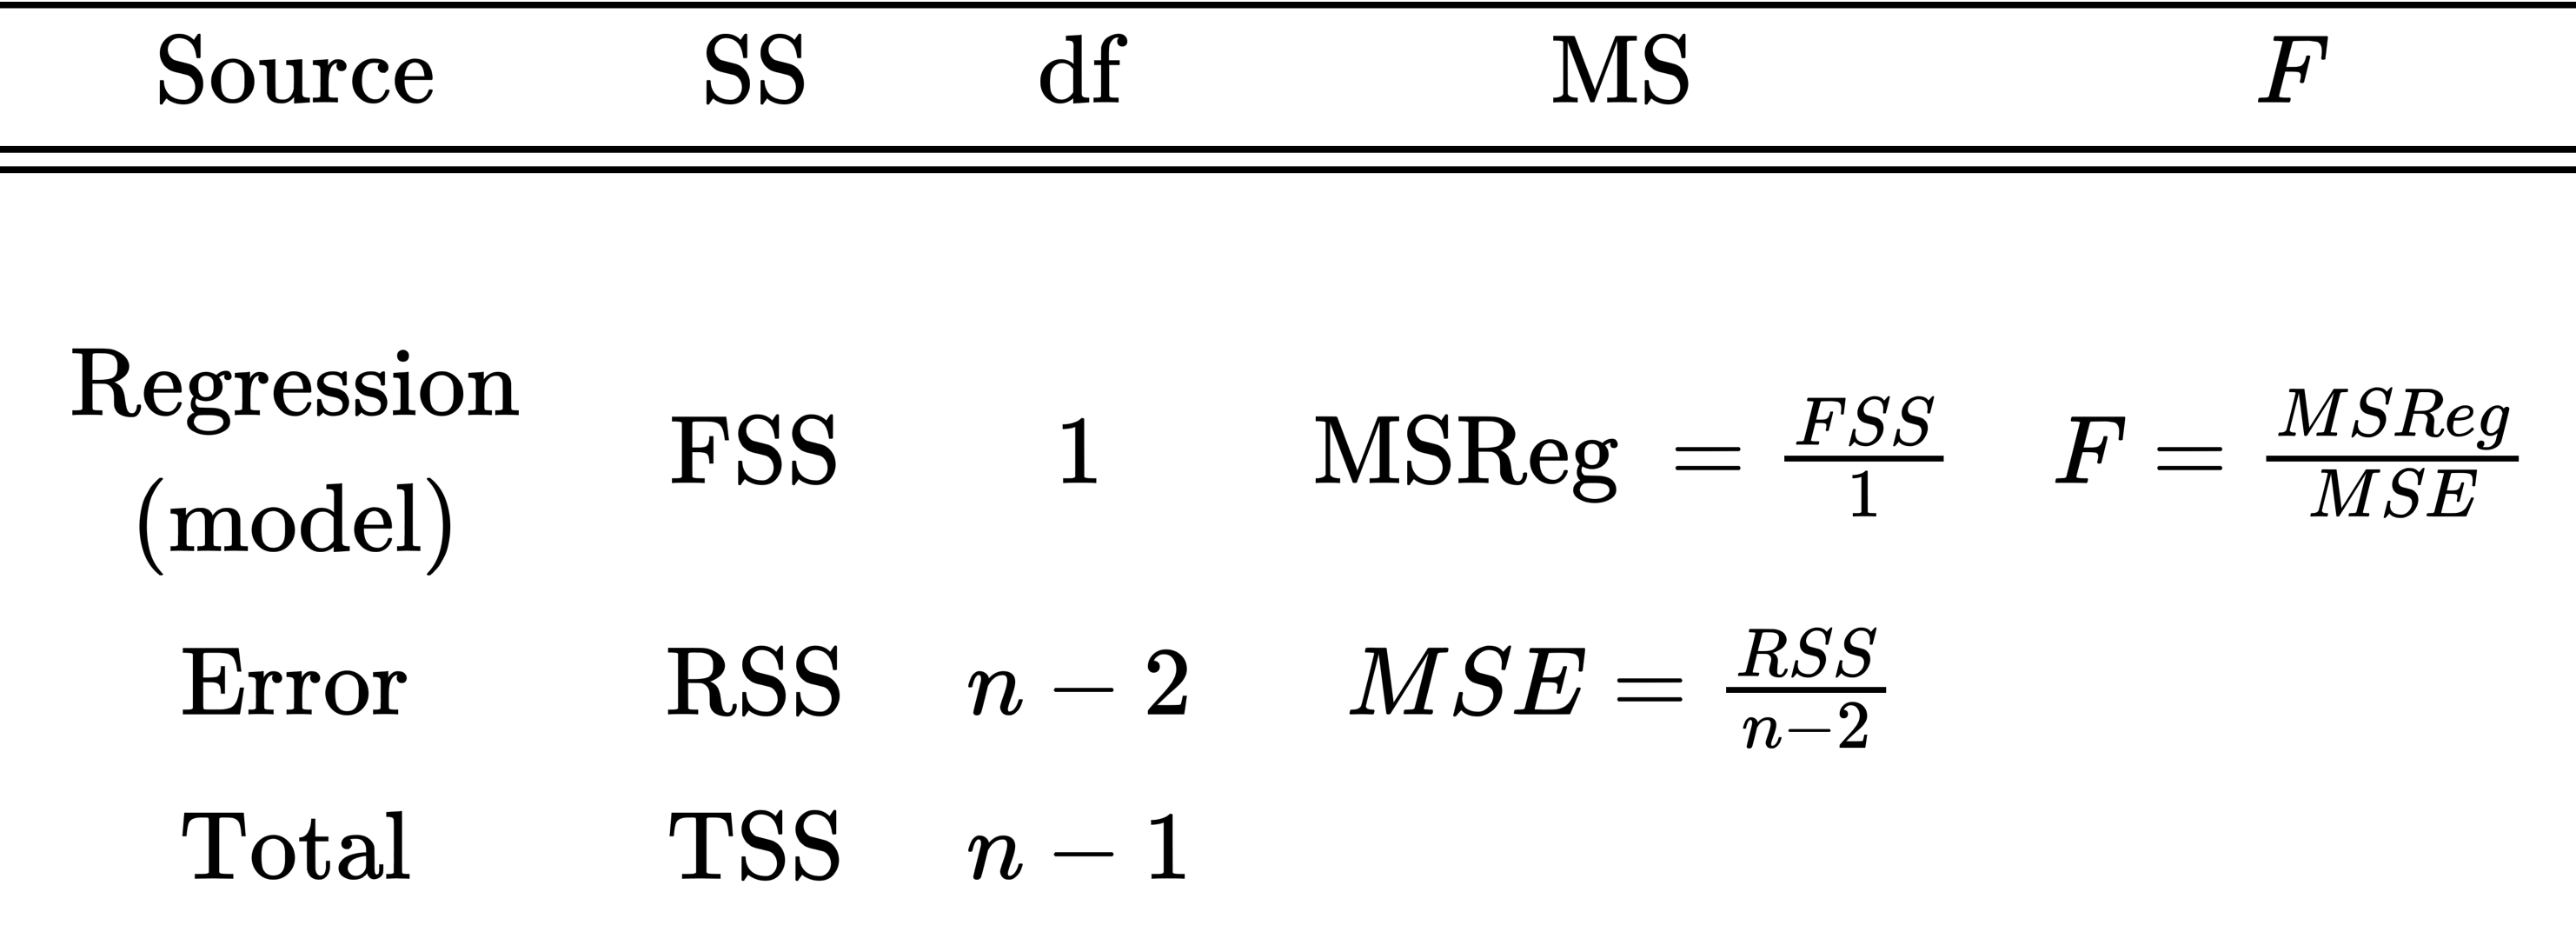
\includegraphics[scale=1]{rendered_image.png}
    \caption{}
    \label{}
\end{figure}\end{center}

\subsubsection{F-Test (equivalent to t-test)}
An alternative way to test for the model parameters is using the $F$ test:
$$
\left\{\begin{array}{l}
H_{0}: \beta_{1}=0 \\
H_{\alpha}: \beta_{1} \neq 0
\end{array}\right.
$$
- Under $H_{0}$, the $F$-test statistic is
$$
F=\frac{\text { MSReg }}{M S E}=\frac{F S S}{R S S /(n-2)} \sim F_{1, n-2}
$$
- It can be shown that the $F$-test statistic is equal to the square of the $t$-test statistic and their $p$-values are the same. So, \textbf{this test is equivalent to the $t$-test before}.

\subsection{Estimation and Prediction}

\subsubsection{Estimation (always reported for a parameter: ${\beta}_0+{\beta}_1x^*=\mathbb{E}(Y|x^*)$)}
1. Estimation: We want to estimate the mean response at $x^*$. This is equivalent to estimate: $\beta_0+\beta_1x^*$\\
2. Accuracy of the estimation: is measured by the expected value of the squared difference between the point estimate and the target.\\
- For estimation the target is $\beta_{0}+\beta_{1} x^{\star}:$
$$
\begin{aligned}
& \mathbb{E}\left(\hat{\beta}_{0}+\hat{\beta}_{1} x^{\star}-\beta_{0}-\beta_{1} x^{\star}\right)^{2} \\
=& \operatorname{Var}\left(\hat{\beta}_{0}+\hat{\beta}_{1} x^{\star}\right) \\
=& \operatorname{Var}\left(\hat{\beta}_{0}\right)+\left(x^{\star}\right)^{2} \operatorname{Var}\left(\hat{\beta}_{1}\right)+2 x^{\star} \operatorname{Cov}\left(\hat{\beta}_{0}, \hat{\beta}_{1}\right) \\
=& \sigma^{2}\left(\frac{1}{n}+\frac{\left(x^{\star}-\bar{x}\right)^{2}}{\sum_{i}\left(x_{i}-\bar{x}\right)^{2}}\right) \\
=& \sigma^{2}\left(\frac{1}{n}+\frac{\left(x^{\star}-\bar{x}\right)^{2}}{S_{x x}}\right)
\end{aligned}
$$

3. Confidence interval: An $(1-\alpha) 100 \%$ Confidence Interval for the Mean Response when $x=x^{\star}$ is given by
$$
\hat{\beta}_{0}+\hat{\beta}_{1} x^{\star} \pm T_{n-2}(\alpha / 2) \hat{\sigma} \sqrt{\frac{1}{n}+\frac{\left(x^{\star}-\bar{x}\right)^{2}}{S_{x x}}}
$$

\subsubsection{Prediction (is reported for the value of a random variable $Y^*$)}
1. Prediction: of an outcome of random variable $Y^*$ at a given value $x^*$ , where $Y^* \sim N( \beta_0 + \beta_1 x^* , \sigma^2 )$\\
2. For prediction the target is $Y^{\star}=\beta_{0}+\beta_{1} x^{\star}+e^{\star}$, where $e^{\star} \sim N\left(0, \sigma^{2}\right)$ This new error $e^{\star}$ is independent of the previous $n$ data points, i.e. is independent of $\left(\hat{\beta}_{0}, \hat{\beta}_{1}\right)$
$$
\begin{aligned}
&\mathbb{E}\left[\left(\hat{\beta}_{0}+\hat{\beta}_{1} x^{\star}-Y^{\star}\right)^{2}\right] \\
&=\mathbb{E}\left[\left(\hat{\beta}_{0}+\hat{\beta}_{1} x^{\star}-\beta_{0}-\beta_{1} x^{\star}-e^{\star}\right)^{2}\right] \\
&=\mathbb{E}\left[\left(\hat{\beta}_{0}+\hat{\beta}_{1} x^{\star}-\beta_{0}-\beta_{1} x^{\star}\right)^{2}\right]+\mathbb{E}\left[\left(e^{\star}\right)^{2}\right] \\
&=\sigma^{2}\left(1+\frac{1}{n}+\frac{\left(x^{\star}-\bar{x}\right)^{2}}{S_{x x}}\right)
\end{aligned}
$$
3. Prediction interval: An $(1-\alpha) 100 \%$ Prediction Interval for $\hat{Y}^{\star}$ when $x=x^{\star}$ is given by
$$
\hat{\beta}_{0}+\hat{\beta}_{1} x^{\star} \pm T_{n-2}(\alpha / 2) \hat{\sigma} \sqrt{1+\frac{1}{n}+\frac{\left(x^{\star}-\bar{x}\right)^{2}}{S_{x x}}}
$$

\subsection{Maximum likelihood estimators with normal error terms}
We start with the statistical model, which is the Gaussian-noise simple linear regression model, defined as follows:\\
1. The distribution of $X$ is arbitrary (and perhaps $X$ is even non-random).\\
2. If $X=x$, then $Y=\beta_{0}+\beta_{1} x+\epsilon$, for some constants ("coefficients", "parameters") $\beta_{0}$ and $\beta_{1}$, and some random noise variable $\epsilon$.\\
3. $\epsilon \sim N\left(0, \sigma^{2}\right)$, and is independent of $X$.\\
4. $\epsilon$ is independent across observations.\\
$$p(y_i|x_i; \beta_0,\beta_1,\sigma^2)=\frac{1}{\sqrt{2\pi\sigma^2}}e^{-\frac{1}{2}(\frac{y_i-(\beta_0+\beta_1x_i)}{\sigma})^2}$$
Given any data set $(x_1, y_1), (x_2, y_2), . . . (x_n, y_n)$, we can now write down the probability density, under the model, of seeing that data:
$$\prod_{i=1}^n p(y_i|x_i; \beta_0,\beta_1,\sigma^2)=\prod_{i=1}^n\frac{1}{\sqrt{2\pi\sigma^2}}e^{-\frac{1}{2}(\frac{y_i-(\beta_0+\beta_1x_i)}{\sigma})^2}=\frac{1}{(2\pi\sigma^2)^{\frac{n}{2}}}e^{-\frac{\sum_{i=1}^n(y_i-(\beta_0+\beta_1x_i))^2}{2\sigma^2}}$$
Take the \textbf{log-likelihood}
$$L(\beta_0,\beta_1,\sigma^2)=-\frac{n}{2}\log{2\pi}-n\log{\sigma}-\frac{1}{2\sigma^2}\sum_{i=1}^n(y_i-(\beta_0+\beta_1x_i))^2$$
Then we can compute the \textbf{Maximum likelihood estimators} $(\hat{\beta}_0,\hat{\beta}_1,\hat{\sigma}^2)$:\\
(1) $(\hat{\beta}_0,\hat{\beta}_1)$,\\
Obviously, maximizing $L(\hat{\beta}_0,\hat{\beta}_1,\hat{\sigma}^2)$ is as same as minimizing $\sum_{i=1}^n(y_i-(\hat{\beta}_0+\hat{\beta}_1x_i))^2$, then the \textbf{Maximum likelihood estimators} is exactly the \textbf{LS estimators}:
$$\begin{aligned}
    &\hat{\beta}_{1}=\frac{\sum_{i=1}^{n}\left(x_{i}-\bar{x}\right)\left(y_{i}-\bar{y}\right)}{\sum_{i=1}^{n}\left(x_{i}-\bar{x}\right)^{2}} \\
    &\hat{\beta}_{0}=\bar{y}-\hat{\beta}_{1} \bar{x}
\end{aligned}$$
(2) $\hat{\sigma}^2$,\\
And the $\hat{\sigma}^2$ is exactly the in-sample mean squared error:
$$\hat{\sigma}^2=\frac{1}{n}\sum_{i=1}^n(y_i-(\hat{\beta}_0+\hat{\beta}_1x_i))^2$$










\section{Multiple Linear Regression}
\subsection{Basic}
$x_{1}, x_{2}, \ldots, x_{p}$ be $p$ predictors of a response $y$.\\
The data will be of the form:
$\begin{array}{ccccc}y_{1} & x_{11} & x_{12} & \cdots & x_{1 p} \\ y_{2} & x_{21} & x_{22} & \cdots & x_{2 p} \\ \vdots & \vdots & \vdots & \ddots & \vdots \\ y_{n} & x_{n 1} & x_{n 2} & \cdots & x_{n p}\end{array}$

Model Equation:
$$
y_{i}=\beta_{1} x_{i 1}+\beta_{2} x_{i 2}+\cdots+\beta_{p} x_{i p}+\varepsilon_{i}, \quad i=1, \ldots, n
$$
where we denote $\mathbf{x}_{\mathbf{i}}=\left(x_{i 1, \ldots, x_{i} p}\right)^{T}$, with $x_{i 1}=1$\\
$\left(\beta_{1}, \beta_{2}, \ldots, \beta_{p} ; \sigma^{2}\right)$ are unknown true parameters.\\
$\beta_{1}$ is the intercept.\\
$\beta_{2}, \beta_{3}, \ldots, \beta_{p}$ are partial slopes.\\
$\sigma^{2}$ is the error variance
\subsubsection{Assumptions of errors}
$\varepsilon_{1}, \varepsilon_{2}, \ldots, \varepsilon_{n}$ are the random errors. They usually assumed to satisfy the same conditions as in simple linear regression:\\
- zero mean: $\mathbb{E}\left(\varepsilon_{i}\right)=0$\\
- uncorrelated: $\left.\operatorname{Cov}\left(\varepsilon_{\mathrm{i}}, \varepsilon_{\mathrm{j}}\right)=0, \mathrm{i} \neq \mathrm{j}\right)$, and\\
- homoscedastic: $\operatorname{Var}\left(\varepsilon_{\mathrm{i}}\right)=\sigma^{2}$ does not depend on $i$ ).

\subsubsection{Matrix Representation}
Matrix Representation of the MLR Model:
$$\begin{array}{cccccc}\mathbf{y}_{n \times 1} & = & \mathbf{X}_{n \times p} & \beta_{p \times 1} & + & \varepsilon_{n \times 1} \\ \uparrow & &\uparrow & \uparrow & &\uparrow \\ \text { Response }& & \text { Design } & \text { Coefficients } & &\text { Error } \\ & & \text { Matrix } & & &\text { Term }\end{array}$$
- $n:$ sample size\\
- $p:$ number of predictors or columns of $X$\\
- By default the intercept is included in the model in which case the first column of $X$ is a vector of 1 's.\\
We set $\mathbb{E}(\varepsilon)=0\text{ and }Cov(\varepsilon)=\sigma^2 \mathbf{I}_n$, then we can infer that
$$\mathbb{E}(y)= \mathbf{X}\beta,\ Cov(y)=\sigma^2 \mathbf{I}_n$$

\subsection{Parameter Estimation $\hat{\beta}=\left(\mathbf{X}^{T} \mathbf{X}\right)^{-1} \mathbf{X}^{T} y$}
- We want to estimate $\beta$, i.e. obtain:
$$
\hat{\beta}=\left(\hat{\beta}_{1}, \hat{\beta}_{2}, \ldots, \hat{\beta}_{p}\right)^{T}
$$
- The LS estimator of $\beta$ minimizes the sum of squared residuals:
$$
R S S=\|y-\mathbf{X} \beta\|^{2}=(y-\mathbf{X} \beta)^{T}(y-\mathbf{X} \beta)
$$
In order to minimize $R S S=(y-\mathbf{X} \beta)^{T}(y-\mathbf{X} \beta)$, we take derivatives with respect to $\beta$ 's and set to zero (as before).\\
$$\frac{\partial R S S}{\partial \beta}=-2 \mathbf{X}_{p \times n}^{T}(y-\mathbf{X} \beta)_{n \times 1}=\mathbf{0}_{p \times 1}$$
$\mathbf{X}^{T}(y-\mathbf{X} \beta)=\mathbf{0} \longrightarrow$ Normal Equations\\
$\left(\mathbf{X}^{T} \mathbf{X}\right) \beta=\mathbf{X}^{T} y$\\
$\hat{\beta}=\left(\mathbf{X}^{T} \mathbf{X}\right)^{-1} \mathbf{X}^{T} y \rightarrow \mathrm{LS}$ Estimators\\
\textbf{Remarks}\\
1. We assume that the rank of $X$ is $p$, i.e. no columns of $X$ is a linear combinations of the other columns of $X$.\\
2. Since $\mathbf{X}$ has rank $p$, the inverse of $\left(\mathbf{X}^{T} \mathbf{X}\right)$ exists.\\
3. if $\left(\mathbf{X}^{T} \mathbf{X}\right)$ is singular the $LS$ solutions is not unique (identifiability problem)

\subsubsection{Fitted Values $\hat{y}_{n \times 1}=\mathbf{H}_{n \times n} y_{n \times 1}$}
$$
\begin{aligned}
\hat{y}_{n \times 1} &=\mathbf{X} \hat{\beta} \\
&=\mathbf{X}\left(\mathbf{X}^{T} \mathbf{X}\right)^{-1} \mathbf{X}^{T} y \\
&=\mathbf{X}\left(\mathbf{X}^{T} \mathbf{X}\right)^{-1} \mathbf{X}^{\top} y\\&=\mathbf{H}_{n \times n} y_{n \times 1}
\end{aligned}
$$
$\mathbf{H}_{n \times n}=\mathbf{X}\left(\mathbf{X}^{T} \mathbf{X}\right)^{-1} \mathbf{X}^{\top}$ is called the hat matrix, since it returns the "y-hat" values.
\subsection{Residuals $\mathbf{r}=(\mathbf{I}-\mathbf{H}) y$, (Sample) error variance $\hat{\sigma}^2=\frac{\mathbf{r}^T \mathbf{r}}{n-p}$}
$$
\mathbf{r}_{n \times 1}=y-\hat{y}=y-\mathbf{H} y=(\mathbf{I}-\mathbf{H}) y
$$
The residuals $\mathbf{r}$ are used to estimate the error variance:
$$
\hat{\sigma}^2=\frac{1}{n-p} \sum_{i} r_{i}^{2}=\frac{\mathbf{r}^T \mathbf{r}}{n-p}=\frac{R S S}{n-p}
$$

\subsection{Properties of residuals}
The LS estimator is the $\beta$ that satisfies the normal equations, that is
$$
\mathbf{X}^{T}(y-\hat{y})=\mathbf{X}^{T}(y-\mathbf{X} \hat{\beta})=\mathbf{0}
$$
This implies the following properties for the residuals, $r_{n \times 1}=y-\mathbf{X} \hat{\beta}$ :
\subsubsection{$\mathbf{X}^{T} \boldsymbol{r}=0$}
1. The cross-products between the residual vector $r$ and each column of $\mathbf{X}$ are zero, i.e.
$$
\begin{aligned}
\mathbf{X}^{T} \boldsymbol{r} &=\mathbf{X}^{T}(\boldsymbol{y}-\mathbf{X} \hat{\boldsymbol{\beta}})=\mathbf{X}^{T} \boldsymbol{y}-\mathbf{X}^{T} \mathbf{X} \hat{\beta} \\
&=\mathbf{X}^{T} \boldsymbol{y}-\left(\mathbf{X}^{T} \mathbf{X}\right)\left(\mathbf{X}^{T} \mathbf{X}\right)^{-1} \mathbf{X}^{T} \boldsymbol{y}=0
\end{aligned}
$$
\subsubsection{$\hat{y}^{T} \boldsymbol{r}=0$}
2. The cross-product between the fitted value $\hat{y}$ and the residual vector $r$ is zero, i.e.
$$
\hat{y}^{T} r=\hat{\beta}^{T} X^{T} r=0
$$
This implies that the residual vector $r$ is \textbf{orthogonal} to each column of $X$ and $\hat{y}$.\\
\subsection{Properties of $\mathbf{H}$}
\subsubsection{$\mathbf{H X}=\mathbf{X}$}
Let $c$ be any linear combination of the columns of $\mathbb{X}$, then
$$
\mathbf{H} c=c
$$
since $\mathbf{H X}=\mathbf{X}\left(\mathbf{X}^{\top} \mathbf{X}\right)^{-1} \mathbf{X}^{T} \mathbf{X}=\mathbf{X}$
\subsubsection{Symmetric: $\mathbf{H}^{T}=\mathbf{H}$}
\textbf{Symmetric}, since $\mathbf{H}^{T}=\left(\mathbf{X}\left(\mathbf{X}^{T} \mathbf{X}\right)^{-1} \mathbf{X}^{T}\right)^{T}=\mathbf{X}\left(\mathbf{X}^{T} \mathbf{X}\right)^{-1} \mathbf{X}^{T}=\mathbf{H}$
\subsubsection{Idempotent: $\mathbf{H H}=\mathbf{H H}^{T}=\mathbf{H}^{\top} \mathbf{H}=\mathbf{H}$}
\textbf{Idempotent}, i.e. $\mathbf{H H}=\mathbf{H H}^{T}=\mathbf{H}^{\top} \mathbf{H}=\mathbf{H} .$ Indeed
$$
\mathbf{H H}=\mathbf{X}\left(\mathbf{X}^{T} \mathbf{X}\right)^{-1} \mathbf{X}^{T} \mathbf{X}\left(\mathbf{X}^{T} \mathbf{X}\right)^{-1} \mathbf{X}^{T}=\mathbf{X}\left(\mathbf{X}^{T} \mathbf{X}\right)^{-1} \mathbf{X}^{T}=\mathbf{H}
$$
\subsubsection{$\mathbf{H}(\mathbf{I}-\mathbf{H})=\mathbf{0}$}
This also implies that $\mathbf{H}(\mathbf{I}-\mathbf{H})=\mathbf{0}_{n \times n}$
\subsubsection{$(\mathbf{I}-\mathbf{H})$ is also symmetric and idempotent}
$$(\mathbf{I}-\mathbf{H})(\mathbf{I}-\mathbf{H})=(\mathbf{I}-\mathbf{H})^T(\mathbf{I}-\mathbf{H})=(\mathbf{I}-\mathbf{H})(\mathbf{I}-\mathbf{H})^T=\mathbf{I}-\mathbf{H}$$
\subsubsection{$\operatorname{trace}(\mathbf{H})=\mathrm{p}$}
$\operatorname{trace}(\mathbf{H})=\mathrm{p}$, the number of $\mathrm{LS}$ coefficients we estimated.

\subsection{Geometric Representation of LS}
\begin{center}\begin{figure}[htbp]
    \centering
    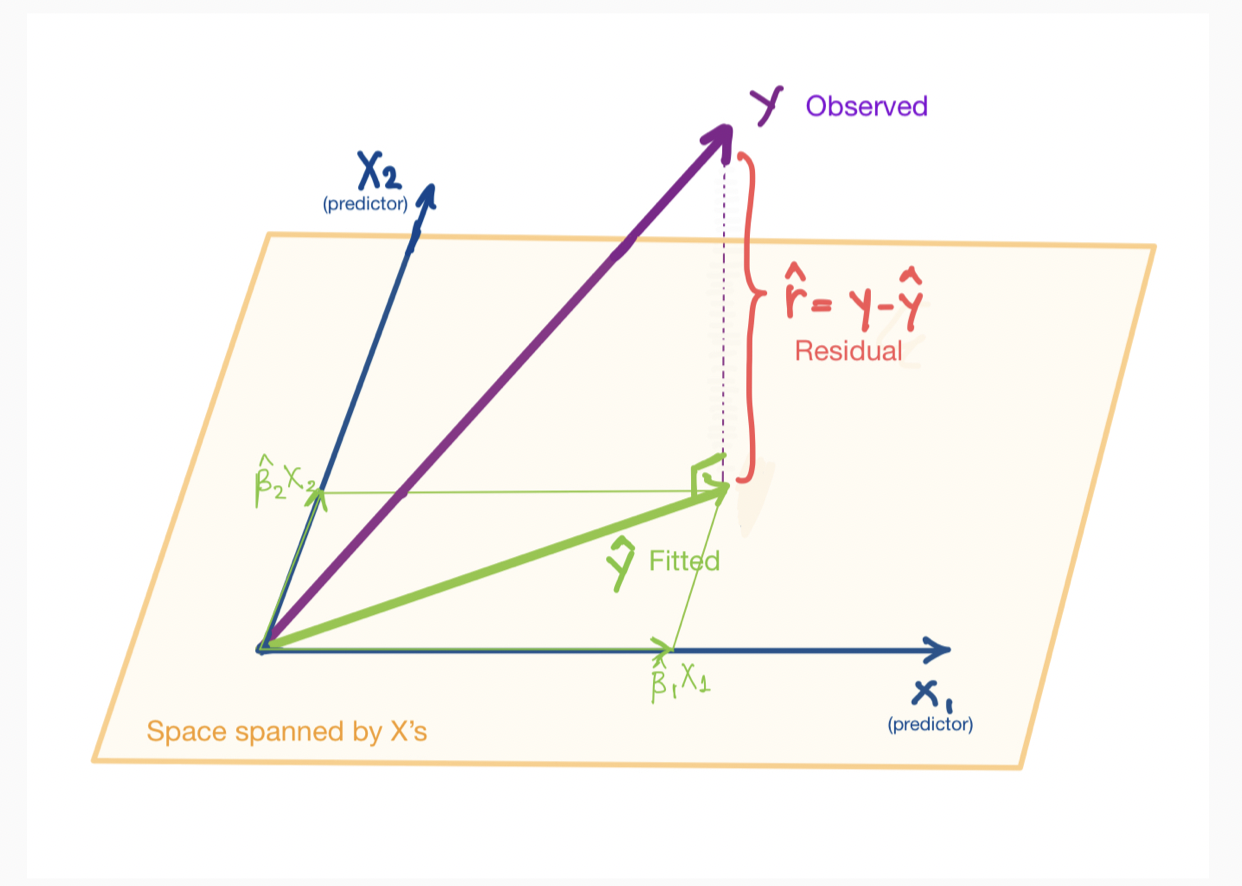
\includegraphics[scale=0.5]{截屏2021-09-05 22.22.04.png}
    \caption{}
    \label{}
\end{figure}\end{center}
\subsubsection{Estimation Space}
- The columns of $\mathbf{X}$ span a $p$-dimensional subspace in $\mathbb{R}^{n}$. This is a subspace that consists of vectors that can be written as linear combinations of the columns of $X$.\\
- The LS squares estimator $\hat{\beta}$ is obtained by minimizing the Euclidean distance between the vectors $\mathbf{y}$ and $\hat{\mathbf{y}}$, i.e. $\|y-\hat{y}\|^{2}$. $\hat{y}$ is the projection of $y$ onto the estimation space.\\
- $\mathbf{H}_{n \times n}$, projection/hat matrix is symmetric, unique, and idempotent.\\
\subsubsection{Error Space}
- The error space is an $(n-p)$-dimensional space that is orthogonal to the estimation space. The projection matrix of the error space is $(\mathbf{I}-\mathbf{H})$.\\
- The residual $\mathbf{r}$ is the projection of $\boldsymbol{y}$ onto the error space, orthogonal to the estimation space. So, $\mathbf{r}$ is orthogonal to any vector in the estimation space, including each column of $X$.\\
- When the intercept is included in the model, then
$$
\sum_{i=1}^{n} r_{i}=0
$$
In general, $\sum_{i=1}^{n} r_{i} X_{i j}=0, j=1, \ldots, p$ due to the normal equations.

\subsection{Coefficient of determination, $R-$Square}
$$
R^{2}=1-\frac{\sum_{i}\left(\hat{y}_{i}-y_{i}\right)^{2}}{\sum_{i}\left(y_{i}-\bar{y}\right)^{2}}=1-\frac{R S S}{T S S}
$$
An equivalent definition is
$$
R^{2}=\frac{\sum_{i}\left(\hat{y}_{i}-\bar{y}\right)^{2}}{\sum_{i}\left(y_{i}-\bar{y}\right)^{2}}
$$
$0 \leq R^{2} \leq 1$

\subsection{Properties of LS Estimators}
\subsubsection{Unbiased: $\mathbb{E}(\hat{\beta})=\beta$}
\begin{equation}
    \begin{aligned}
        \mathbb{E}(\hat{\beta})&=\mathbb{E}(\left(\mathbf{X}^{T} \mathbf{X}\right)^{-1} \mathbf{X}^{T} y)=\left(\mathbf{X}^{T} \mathbf{X}\right)^{-1} \mathbf{X}^{T} \mathbb{E}(y)\\
        &=\left(\mathbf{X}^{T} \mathbf{X}\right)^{-1} \mathbf{X}^{T}\mathbf{X}\beta=\beta
    \end{aligned}
    \nonumber
\end{equation}

\subsubsection{Variance-Covariance Matrix of $\hat{\beta}$: $\operatorname{Cov}(\hat{\beta})=\sigma^{2}\left(\mathbf{X}^{T} \mathbf{X}\right)^{-1}$}
$$\begin{aligned} \operatorname{Cov}(\hat{\beta}) &=\left(\mathbf{X}^{T} \mathbf{X}\right)^{-1} \mathbf{X}^{T} \operatorname{Cov}(\mathbf{y})\left(\left(\mathbf{X}^{\top} \mathbf{X}\right)^{-1} \mathbf{X}^{\top}\right)^{\top} \\ &=\left(\mathbf{X}^{T} \mathbf{X}\right)^{-1} \mathbf{X}^{T} \sigma^{2} \mathbf{X}\left(\mathbf{X}^{\top} \mathbf{X}\right)^{-1} \\ &=\sigma^{2}\left(\mathbf{X}^{T} \mathbf{X}\right)^{-1} \mathbf{X}^{\top} \mathbf{X}\left(\mathbf{X}^{T} \mathbf{X}\right)^{-1} \\ &=\sigma^{2}\left(\mathbf{X}^{T} \mathbf{X}\right)^{-1} \end{aligned}$$
$$se(\hat{\beta}_i)=\hat{\sigma}\sqrt{((\mathbf{X}^T\mathbf{X})^{-1})_{ii}}$$


\subsubsection{$\hat{y}$: $\mathbb{E}(\hat{y})=\mathbf{X}\beta$, $Cov(\hat{y})=\sigma^2 \mathbf{H}$}
\begin{equation}
    \begin{aligned}
        &\mathbb{E}(\hat{y})=\mathbb{E}(\mathbf{X}\left(\mathbf{X}^{T} \mathbf{X}\right)^{-1} \mathbf{X}^{\top}y)=\mathbf{X}\left(\mathbf{X}^{T} \mathbf{X}\right)^{-1} \mathbf{X}^{\top}\mathbf{X}\beta=\mathbf{X}\beta\\
        &Cov(\hat{y})=Cov(\mathbf{H}y)=\mathbf{H}Cov(y)\mathbf{H}^T=\sigma^2\mathbf{H}\mathbf{H}^T=\sigma^2\mathbf{H}
    \end{aligned}
    \nonumber
\end{equation}
\subsubsection{$\mathbf{r}$: $\mathbb{E}(\mathbf{r})=0$, $Cov(\mathbf{r})=\sigma^2 (\mathbf{I}_n-\mathbf{H})$}
\begin{equation}
    \begin{aligned}
        &\mathbb{E}(\mathbf{r})=\mathbb{E}(y-\hat{y})=0\\
        &Cov(\mathbf{r})=Cov(y-\hat{y})=Cov((\mathbf{I}-\mathbf{H})y)=\sigma^2(\mathbf{I}-\mathbf{H})(\mathbf{I}-\mathbf{H})^T=\sigma^2(\mathbf{I}-\mathbf{H})
    \end{aligned}
    \nonumber
\end{equation}
\subsubsection{$\mathbb{E}(\hat{\sigma}^2)=\sigma^2$}
$$\mathbb{E}(\hat{\sigma}^2)=\frac{1}{n-p}\mathbb{E}(\mathbf{r}^T \mathbf{r})=\frac{1}{n-p}\sigma^2(n-p)=\sigma^2$$
$n-p$来自于: 有$p$个元素在H对角中为$1$,其余为$0$,所以$\mathbf{I}_n-\mathbf{H}$对角中有$n-p$个1。所以只有$n-p$个$r_i^2=\sigma^2$
$$\frac{\mathbf{r}^T \mathbf{r}}{\sigma^2}=\frac{RSS}{\sigma^2}\sim \chi^2_{n-p}$$

\subsection{The Gauss-Markov Theorem: LS estimator is the \textbf{BLUE}(best linear unbiased estimator)}
If the errors are 1. Mean zero, 2. umcorrelated, 3. homoscedastic, the LS estimators have \textbf{the lowest variance within the class of linear estimators.}\\
Suppose we are interested in estimating a linear combination of $\beta$ of the form:
$$\theta=\mathbf{c}^T\beta=\sum_{j=1}^pc_j\beta_j$$
LS estimators:
$$\hat{\theta}_{LS}=\mathbf{c}^T\hat{\beta}=\mathbf{c}^T \left(\mathbf{X}^{T} \mathbf{X}\right)^{-1} \mathbf{X}^{T} y$$
This is a \textbf{linear} (linear combination of $y_1,y_2,...,y_n$) and \textbf{unbiased estimator} of $\theta$. Its mean square error can be calculated as:
$$
MSE( \hat{\theta}_{LS} ) = \mathbb{E}( \hat{\theta}_{LS} − \theta)^2 = Var( \hat{\theta}_{LS})$$
\begin{theorem}[Gauss-Markov Theorem]
    $\hat{\theta}_{LS}=\mathbf{c}^T\hat{\beta}$ is the \textbf{BLUE}(best linear unbiased estimator) of the parameter $\mathbf{c}^T\beta$ for any vector $\mathbf{c}\in \mathbb{R}^p$
\end{theorem}

\subsection{Maximum Likelihood Estimation, Distribution of LS estimates}
\subsubsection{$\mathbf{y} \sim \mathbf{N}_{n}\left(\mathbf{X} \beta, \sigma^{2} \mathbf{I}\right)$}
Recall the normality assumption for the regression model:
$$
y_{i}=\mathbf{x}_{i}^{T} \beta+\varepsilon_{i},\quad i=1, \ldots, n, \text { with } \varepsilon_{i} \sim N\left(0, \sigma^{2}\right)
$$
This implies that $\mathbf{y} \sim \mathbf{N}_{n}\left(\mathbf{X} \beta, \sigma^{2} \mathbf{I}\right)$

\subsubsection{LS estimator is the Maximum Likelihood Estimator (MLE)}
We can show that the likelihood function can be written as:
$$
L\left(\beta, \sigma^{2} \mid \mathbf{y}\right) \propto \frac{R S S}{n}^{-\frac{n}{2}}
$$
The value of $\beta$ that maximizes the Likelihood function is \textit{the Maximum Likelihood Estimator (MLE)} of $\beta$. This estimator is equal to the LS estimate of $\beta$.
\subsubsection{$\hat{\beta}\sim \mathbf{N}_{\mathbf{p}}\left(\beta, \sigma^{2}\left(\mathbf{X}^{\top} \mathbf{X}\right)^{-1}\right)$, $\hat{\mathbf{y}}\sim\mathbf{N}_{\mathbf{n}}\left(\mathbf{X} \beta, \sigma^{2} \mathbf{H}\right)$, $\hat{\mathbf{r}}\sim \mathbf{N}_{\mathbf{n}}\left(\mathbf{0}, \sigma^{2}\left(\mathbf{I}_{\mathbf{n}}-\mathbf{H}\right)\right)$}
Recall the assumption for the linear regression model:
$$
\mathbf{y} \sim \mathbf{N}_{\mathbf{n}}\left(\mathbf{X} \beta, \sigma^{2} \mathbf{I}\right)
$$
Any affine transformation of $\mathbf{y}$ will also have a Normal distribution $^{2}$.
We can show that:
$$
\begin{gathered}
\hat{\beta}=\left(\mathbf{X}^{\top} \mathbf{X}\right)^{-1} \mathbf{X}^{\top} \mathbf{y} \sim \mathbf{N}_{\mathbf{p}}\left(\beta, \sigma^{2}\left(\mathbf{X}^{\top} \mathbf{X}\right)^{-1}\right) \\
\hat{\mathbf{y}}=\mathbf{H} \mathbf{y} \sim \mathbf{N}_{\mathbf{n}}\left(\mathbf{X} \beta, \sigma^{2} \mathbf{H}\right) \\
\hat{\mathbf{r}}=\left(\mathbf{I}_{\mathbf{n}}-\mathbf{H}\right) \mathbf{y} \sim \mathbf{N}_{\mathbf{n}}\left(\mathbf{0}, \sigma^{2}\left(\mathbf{I}_{\mathbf{n}}-\mathbf{H}\right)\right)
\end{gathered}
$$
\subsection{$\mathbf{r}$ Residuals’ Properties}
\subsubsection{$\mathbf{r}\in \mathbb{R}^{n-p}$}
Although $\mathbf{r}$ is a vector of dimension $n$, it always lies in a subspace of dimension $(n − p)$.
\subsubsection{$\hat{\sigma}^{2}\sim\sigma^{2} \frac{\chi_{n-p}^{2}}{n-p}$}
r behaves like a random vector with a distribution $\mathbf{N}_{n-p}\left(\mathbf{0}, \sigma^{2} \mathbf{I}_{n-p}\right)$, so we have:
$$
\hat{\sigma}^{2}=\frac{\|\mathbf{r}\|^{2}}{n-p} \sim \sigma^{2} \frac{\chi_{n-p}^{2}}{n-p}
$$
\subsubsection{$\hat{\mathbf{y}}$ and $\boldsymbol{r}$ are independent}
It can be show that $\hat{\mathbf{y}}$ and $\boldsymbol{r}$ are uncorrelated since they are in orthogonal spaces. Since they also have a joint normal distribution, they are independent.

\subsection{Testing Predictors (Coefficients)}
\subsubsection{Testing a Single Predictor $H_0: \beta_j=0$: $t-$test}
Suppose you have a $p$ predictors in your regression model and you want to test the hypothesis:
$$
H_{0}: \beta_{j}=c \text { vs. } H_{\alpha}: \beta_{j} \neq c
$$
- The t-test statistic we use is:
$$
t=\frac{\hat{\beta}_{j}-c}{s e\left(\hat{\beta}_{j}\right)}=\frac{\hat{\beta}_{j}-c}{\hat{\sigma} \sqrt{\left[\left(\mathbf{X}^{\top} \mathbf{X}\right)^{-1}\right]_{j j}}} \sim T_{n-p}
$$
under the null hypothesis $H_{0}$.\\
- p-value $=2 \times$ the area under the curve of a $T_{n-p}$ distribution more extreme than the observed statistic.\\
- The $p$-value returned by the $I m$ function command is for $c=0$.
\subsubsection{Review the degree of freedom}
The degrees of freedom of a $t$-test are determined by the \underline{denominator} of the estimated variance $\hat{\sigma}^{2}$. Consider the following situations:\\
- In STAT 400: Test for $\theta=\alpha$, where $Z_{1}, \ldots, Z_{n} \sim \mathcal{N}\left(\theta, \sigma^{2}\right)$
$$
\frac{\hat{\theta}-\alpha}{\operatorname{se}(\hat{\theta})}=\frac{\overline{\mathbf{Z}}-\alpha}{\sqrt{\hat{\sigma}^{2} / n}} \sim T_{n-1}, \quad \hat{\sigma}^{2}=\frac{\sum_{i}\left(Z_{i}-\bar{Z}\right)^{2}}{n-1}
$$
- In SLR: Test for $\beta_{1}=c$, we have
$$
\frac{\hat{\beta}_{1}-c}{\operatorname{se}\left(\hat{\beta}_{1}\right)}=\frac{\hat{\beta}_{1}-c}{\hat{\sigma} / \sqrt{S_{X X}}} \sim T_{n-2},\quad \hat{\sigma}^{2}=\frac{R S S}{n-2}
$$
- In $M L R$ with $p$ predictors (including the intercept): Test for $\beta_{j}=c$,
$$
\frac{\hat{\beta}_{j}-c}{\operatorname{se}\left(\hat{\beta}_{j}\right)}=\frac{\hat{\beta}_{j}-c}{\hat{\sigma} \sqrt{\left[\left(\mathbf{X}^{T} \mathbf{X}\right)^{-1}\right]_{j j}}} \sim T_{n-p}, \quad\hat{\sigma}^{2}=\frac{R S S}{n-p}
$$

\subsubsection{Testing all predictors: $F-$test}
Testing all predictors
$$
\left\{\begin{array}{l}
H_{0}: \beta_{2}=\beta_{3}=\ldots=\beta_{p}=0 \\
H_{a}: \beta_{j} \neq 0, \quad \text { for some } j, j=2, \ldots, p
\end{array}\right.
$$
- Under the Null hypothesis, the test statistic:
$$
\begin{aligned}
F &=\frac{F S S\left(X_{2}, \ldots, X_{p}\right)}{p-1} \div \frac{R S S\left(X_{2}, \ldots, X_{p}\right)}{n-p} \\
&=\frac{M S(R e g)}{M S(\text { Error })} \sim F_{p-1, n-p}
\end{aligned}
$$
Large values of $F$ lead to conclusion $H_{\alpha}$.\\
- This is the overall $F$ test of whether or not there is a regression relation between the response variable $Y$ and the set of $X$ variables.
\begin{center}\begin{figure}[htbp]
    \centering
    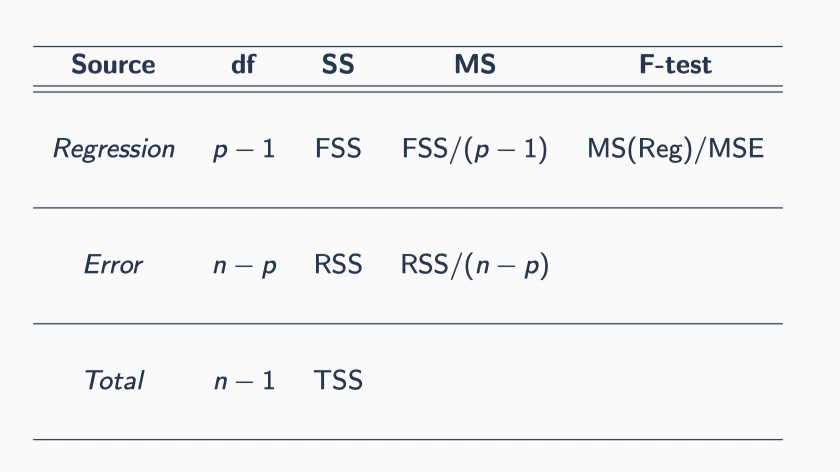
\includegraphics[scale=0.8]{Lec0601.png}
    \caption{}
    \label{}
\end{figure}\end{center}
\subsubsection{Partial $F-$test}
In general, consider the following partition of the design matrix into two sub-matrices $\mathbf{X}_{1}$ and $\mathbf{X}_{2}$, that is
$$
\mathbf{X}_{n \times p}=\left(\mathbf{X}_{1 n \times(p-q)}, \mathbf{X}_{2 n \times q}\right)
$$
The corresponding partition of the regression parameter is:
$$
\beta^{T}=\left(\beta_{1}^{T}, \beta_{2}^{T}\right)
$$
where $\beta_{1}$ is $(p-q) \times 1$ and $\beta_{2}$ is $q \times 1$\\
This partition is used to test the hypothesis:
$$
\left\{\begin{array}{l}
H_{0}: \beta_{2}=\mathbf{0}, \text { i.e., } \quad \mathbf{y}=\mathbf{X}_{1} \beta_{1}+\text { error } \\
H_{\alpha}: \beta_{2} \neq \mathbf{0}, \text { i.e., }\quad \mathbf{y}=\mathbf{X}_{1} \beta_{1}+\mathbf{X}_{2} \beta_{2}+\text { error }
\end{array}\right.
$$
To test this hypothesis, the test statistic is:
$$
F=\frac{\left(R S S_{0}-R S S_{\alpha}\right) / q}{R S S_{\alpha} /(n-p)} \sim F_{q, n-p}
$$
where \textbf{$R R S_{0}=$ Residual sum of squares for the model under $H_{0}$ ; $R R S_{a}=$ Residual sum of squares for the model under $H_{\alpha}$}

\textbf{Numerator}: variation in the data not explained by the reduced model, but explained by the full model.

\textbf{Denominator}: variation in the data not explained by the full model (i.e., not explained by either model), which is used to estimate the error variance.

\textit{Reject $H_{0}$, if $F$ test statistic is large}, that is, the variation missed by the reduced model, when being compared with the error variance, is significantly large.

F-test statistic can be rewirtten:
$$F=\frac{\left(R S S_{0}-R S S_{\alpha}\right) / q}{R S S_{\alpha} /(n-p)}=\frac{((1-R_R^2)-(1-R_F^2))/(df_F-df_R)}{(1-R_F^2)/df_F}=\frac{(R_F^2-R_R^2)/(df_R-df_F)}{(1-R_F^2)/df_F}$$
Note that this test statistic is not appropriate when the full and reduced regression models do not contain the intercept term $\beta_0$ .

\subsection{Permutation Tests (When the normal distribution hypothesis doesn't hold)}
The distribution of the data is \textit{unknown}.
- A test statistic is a function of the data; denote it $g($ data $)$.\\
- The test statistic tends to take extreme values under the alternative hypothesis $H_{\alpha}$.
\subsubsection{Procedure}
Procedure to conduct a permutation test\\
1. Form the test statistic $g($ data $)$ which tends to take extreme values under the alternative hypothesis.\\
2. Evaluate the test statistic on the observed data, denoted by $g_{0}$.\\
3. Find the distribution of $g($ data $)$, when data are generated from $H_{0}$.\\
4. Calculate the $p$-value, that is the following probability:
\begin{center}
    $\mathbb{P}\left(g(\right.$ data $)$ is more extreme than the observed $g_{0} \mid$ data $\left.\sim H_{0}\right)$
\end{center}

\subsubsection{Calculation of the p-value: Monte Carlo method}
We can obtain an approximation of $\mathbb{E}(Y)$ as follows:\\
1. Generate $N=1000$ samples from this distribution, $Y_{1}, \ldots, Y_{N}$\\
2. Approximate the mean by
$$
\mathbb{E}(Y) \approx \frac{1}{N} \sum_{i=1}^{N} Y_{i}
$$
That is, population mean $\approx$ sample mean (when $N$ is large).\\

This method also works if we want to approximate the expected value of a \textit{function} of a random variable:
$$
\mathbb{E}(f(Y)) \approx \frac{1}{N} \sum_{i=1}^{N} f\left(Y_{i}\right)
$$

\subsection{Confidence Intervals for $\beta_j$, Confidence Region for $\beta$}
\subsubsection{Confidence Intervals for $\beta_j$}
Recall that
$$\hat{\beta}=\left(\mathbf{X}^{\top} \mathbf{X}\right)^{-1} \mathbf{X}^{\top} \mathbf{y} \sim \mathbf{N}_{\mathbf{p}}\left(\beta, \sigma^{2}\left(\mathbf{X}^{\top} \mathbf{X}\right)^{-1}\right)$$
An $(1-\alpha)100\%$ CI(Confidence Interval) for $\beta_j$ can be written as
$$(\hat{\beta}_j \pm T_{n-p}(\frac{\alpha}{2})se(\hat{\beta}_j))=(\hat{\beta}_j \pm T_{n-p}(\frac{\alpha}{2})\hat{\sigma}\sqrt{[\left(\mathbf{X}^{\top} \mathbf{X}\right)^{-1}]_{jj}})$$
\subsubsection{Confidence Region for $\beta$}
$\beta$ is the entire vector,
$$\beta-\hat{\beta}\sim\mathbf{N}_{\mathbf{p}}\left(0, \sigma^{2}\left(\mathbf{X}^{\top} \mathbf{X}\right)^{-1}\right)$$
Thus the quadratic form:
$$\frac{(\beta-\hat{\beta})^T \mathbf{X}^T \mathbf{X}(\beta-\hat{\beta})}{p \hat{\sigma}^2}\sim F_{p,n-p}$$
We can construct a $(1-\alpha)100\%$ confidence region for $\beta$ to be all the points in the following ellipsoid,
$$\frac{(\beta-\hat{\beta})^T \mathbf{X}^T \mathbf{X}(\beta-\hat{\beta})}{p \hat{\sigma}^2}<F(\alpha; p,n-p)$$
Where $F(\alpha; p,n-p)$ is defined to be the point such that $$\mathbb{P}(F_{p,n-p}>F(\alpha; p,n-p))=\alpha$$
\begin{center}\begin{figure}[htbp]
    \centering
    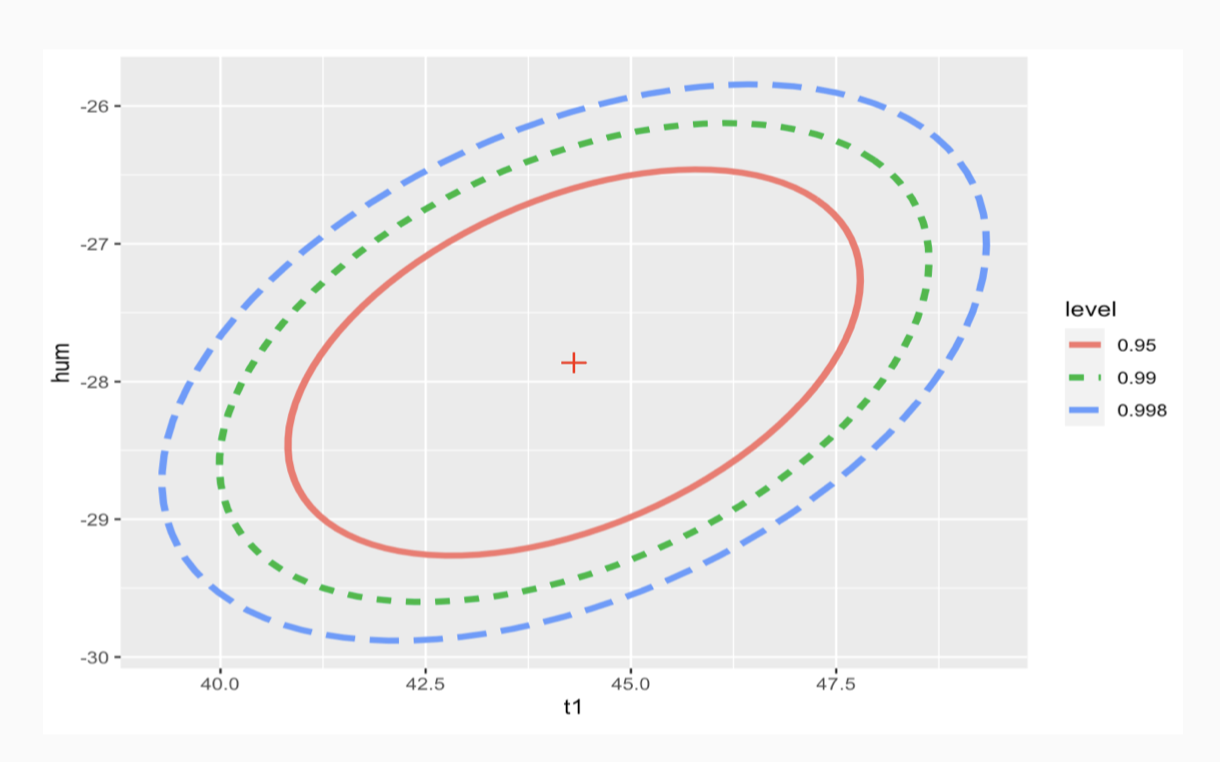
\includegraphics[scale=0.5]{Lec0701.png}
    \caption{}
    \label{}
\end{figure}\end{center}

\subsection{Confidence/Prediction Intervals for New Observations}
Set $\mathbb{E}(Y|x^*)=\mu^*=(x^*)^T\beta$
\subsubsection{Confidence Interval for $\mu^*=(x^*)^T\beta$}
The Gauss-Markov theorem tells us that the BLUE (Best Linear Unbiased Estimate) of $\mu^*$ is:
$$\hat{\mu}^*=(x^*)^T \hat{\beta}=(x^*)^T(X^TX)^{-1}X^Ty$$
Then,
\begin{equation}
    \begin{aligned}
        Var(\hat{\mu}^*)=[((x^*)^T\hat{\beta})-((x^*)^T\beta)]
    \end{aligned}
    \nonumber
\end{equation}
$$se(\hat{\mu}^*)=\hat{\sigma}\sqrt{(x^*)^T(X^TX)^{-1}X^Tx^*}$$
A confidence interval for $\mu^*$ is:
$$\hat{\mu}^*\pm T_{n-p}(\frac{\alpha}{2})se(\hat{\mu}^*)$$
\subsubsection{Prediction Interval for $y^*=(x^*)^T\beta+e^*$}
The best estimate for $y^*$ at a future observation $x^*$ is also
$$\hat{y}^*=(x^*)^T \hat{\beta}$$


























































\end{document}